% Options for packages loaded elsewhere
\PassOptionsToPackage{unicode}{hyperref}
\PassOptionsToPackage{hyphens}{url}
%
\documentclass[
]{book}
\usepackage{lmodern}
\usepackage{amssymb,amsmath}
\usepackage{ifxetex,ifluatex}
\ifnum 0\ifxetex 1\fi\ifluatex 1\fi=0 % if pdftex
  \usepackage[T1]{fontenc}
  \usepackage[utf8]{inputenc}
  \usepackage{textcomp} % provide euro and other symbols
\else % if luatex or xetex
  \usepackage{unicode-math}
  \defaultfontfeatures{Scale=MatchLowercase}
  \defaultfontfeatures[\rmfamily]{Ligatures=TeX,Scale=1}
\fi
% Use upquote if available, for straight quotes in verbatim environments
\IfFileExists{upquote.sty}{\usepackage{upquote}}{}
\IfFileExists{microtype.sty}{% use microtype if available
  \usepackage[]{microtype}
  \UseMicrotypeSet[protrusion]{basicmath} % disable protrusion for tt fonts
}{}
\makeatletter
\@ifundefined{KOMAClassName}{% if non-KOMA class
  \IfFileExists{parskip.sty}{%
    \usepackage{parskip}
  }{% else
    \setlength{\parindent}{0pt}
    \setlength{\parskip}{6pt plus 2pt minus 1pt}}
}{% if KOMA class
  \KOMAoptions{parskip=half}}
\makeatother
\usepackage{xcolor}
\IfFileExists{xurl.sty}{\usepackage{xurl}}{} % add URL line breaks if available
\IfFileExists{bookmark.sty}{\usepackage{bookmark}}{\usepackage{hyperref}}
\hypersetup{
  pdftitle={Microeconomics},
  pdfauthor={Noah Love},
  hidelinks,
  pdfcreator={LaTeX via pandoc}}
\urlstyle{same} % disable monospaced font for URLs
\usepackage{color}
\usepackage{fancyvrb}
\newcommand{\VerbBar}{|}
\newcommand{\VERB}{\Verb[commandchars=\\\{\}]}
\DefineVerbatimEnvironment{Highlighting}{Verbatim}{commandchars=\\\{\}}
% Add ',fontsize=\small' for more characters per line
\usepackage{framed}
\definecolor{shadecolor}{RGB}{248,248,248}
\newenvironment{Shaded}{\begin{snugshade}}{\end{snugshade}}
\newcommand{\AlertTok}[1]{\textcolor[rgb]{0.94,0.16,0.16}{#1}}
\newcommand{\AnnotationTok}[1]{\textcolor[rgb]{0.56,0.35,0.01}{\textbf{\textit{#1}}}}
\newcommand{\AttributeTok}[1]{\textcolor[rgb]{0.77,0.63,0.00}{#1}}
\newcommand{\BaseNTok}[1]{\textcolor[rgb]{0.00,0.00,0.81}{#1}}
\newcommand{\BuiltInTok}[1]{#1}
\newcommand{\CharTok}[1]{\textcolor[rgb]{0.31,0.60,0.02}{#1}}
\newcommand{\CommentTok}[1]{\textcolor[rgb]{0.56,0.35,0.01}{\textit{#1}}}
\newcommand{\CommentVarTok}[1]{\textcolor[rgb]{0.56,0.35,0.01}{\textbf{\textit{#1}}}}
\newcommand{\ConstantTok}[1]{\textcolor[rgb]{0.00,0.00,0.00}{#1}}
\newcommand{\ControlFlowTok}[1]{\textcolor[rgb]{0.13,0.29,0.53}{\textbf{#1}}}
\newcommand{\DataTypeTok}[1]{\textcolor[rgb]{0.13,0.29,0.53}{#1}}
\newcommand{\DecValTok}[1]{\textcolor[rgb]{0.00,0.00,0.81}{#1}}
\newcommand{\DocumentationTok}[1]{\textcolor[rgb]{0.56,0.35,0.01}{\textbf{\textit{#1}}}}
\newcommand{\ErrorTok}[1]{\textcolor[rgb]{0.64,0.00,0.00}{\textbf{#1}}}
\newcommand{\ExtensionTok}[1]{#1}
\newcommand{\FloatTok}[1]{\textcolor[rgb]{0.00,0.00,0.81}{#1}}
\newcommand{\FunctionTok}[1]{\textcolor[rgb]{0.00,0.00,0.00}{#1}}
\newcommand{\ImportTok}[1]{#1}
\newcommand{\InformationTok}[1]{\textcolor[rgb]{0.56,0.35,0.01}{\textbf{\textit{#1}}}}
\newcommand{\KeywordTok}[1]{\textcolor[rgb]{0.13,0.29,0.53}{\textbf{#1}}}
\newcommand{\NormalTok}[1]{#1}
\newcommand{\OperatorTok}[1]{\textcolor[rgb]{0.81,0.36,0.00}{\textbf{#1}}}
\newcommand{\OtherTok}[1]{\textcolor[rgb]{0.56,0.35,0.01}{#1}}
\newcommand{\PreprocessorTok}[1]{\textcolor[rgb]{0.56,0.35,0.01}{\textit{#1}}}
\newcommand{\RegionMarkerTok}[1]{#1}
\newcommand{\SpecialCharTok}[1]{\textcolor[rgb]{0.00,0.00,0.00}{#1}}
\newcommand{\SpecialStringTok}[1]{\textcolor[rgb]{0.31,0.60,0.02}{#1}}
\newcommand{\StringTok}[1]{\textcolor[rgb]{0.31,0.60,0.02}{#1}}
\newcommand{\VariableTok}[1]{\textcolor[rgb]{0.00,0.00,0.00}{#1}}
\newcommand{\VerbatimStringTok}[1]{\textcolor[rgb]{0.31,0.60,0.02}{#1}}
\newcommand{\WarningTok}[1]{\textcolor[rgb]{0.56,0.35,0.01}{\textbf{\textit{#1}}}}
\usepackage{longtable,booktabs}
% Correct order of tables after \paragraph or \subparagraph
\usepackage{etoolbox}
\makeatletter
\patchcmd\longtable{\par}{\if@noskipsec\mbox{}\fi\par}{}{}
\makeatother
% Allow footnotes in longtable head/foot
\IfFileExists{footnotehyper.sty}{\usepackage{footnotehyper}}{\usepackage{footnote}}
\makesavenoteenv{longtable}
\usepackage{graphicx,grffile}
\makeatletter
\def\maxwidth{\ifdim\Gin@nat@width>\linewidth\linewidth\else\Gin@nat@width\fi}
\def\maxheight{\ifdim\Gin@nat@height>\textheight\textheight\else\Gin@nat@height\fi}
\makeatother
% Scale images if necessary, so that they will not overflow the page
% margins by default, and it is still possible to overwrite the defaults
% using explicit options in \includegraphics[width, height, ...]{}
\setkeys{Gin}{width=\maxwidth,height=\maxheight,keepaspectratio}
% Set default figure placement to htbp
\makeatletter
\def\fps@figure{htbp}
\makeatother
\setlength{\emergencystretch}{3em} % prevent overfull lines
\providecommand{\tightlist}{%
  \setlength{\itemsep}{0pt}\setlength{\parskip}{0pt}}
\setcounter{secnumdepth}{5}
\usepackage{booktabs}
\usepackage{amsthm}
\makeatletter
\def\thm@space@setup{%
  \thm@preskip=8pt plus 2pt minus 4pt
  \thm@postskip=\thm@preskip
}
\makeatother
\usepackage[]{natbib}
\bibliographystyle{apalike}

\title{Microeconomics}
\author{Noah Love}
\date{2020-09-15}

\begin{document}
\maketitle

{
\setcounter{tocdepth}{1}
\tableofcontents
}
\hypertarget{introduction}{%
\chapter{Introduction}\label{introduction}}

Hello this is a test

\hypertarget{intro}{%
\chapter{Introduction}\label{intro}}

You can label chapter and section titles using \texttt{\{\#label\}} after them, e.g., we can reference Chapter \ref{intro}. If you do not manually label them, there will be automatic labels anyway, e.g., Chapter \ref{methods}.

Figures and tables with captions will be placed in \texttt{figure} and \texttt{table} environments, respectively.

\begin{Shaded}
\begin{Highlighting}[]
\KeywordTok{par}\NormalTok{(}\DataTypeTok{mar =} \KeywordTok{c}\NormalTok{(}\DecValTok{4}\NormalTok{, }\DecValTok{4}\NormalTok{, }\FloatTok{.1}\NormalTok{, }\FloatTok{.1}\NormalTok{))}
\KeywordTok{plot}\NormalTok{(pressure, }\DataTypeTok{type =} \StringTok{'b'}\NormalTok{, }\DataTypeTok{pch =} \DecValTok{19}\NormalTok{)}
\end{Highlighting}
\end{Shaded}

\begin{figure}

{\centering 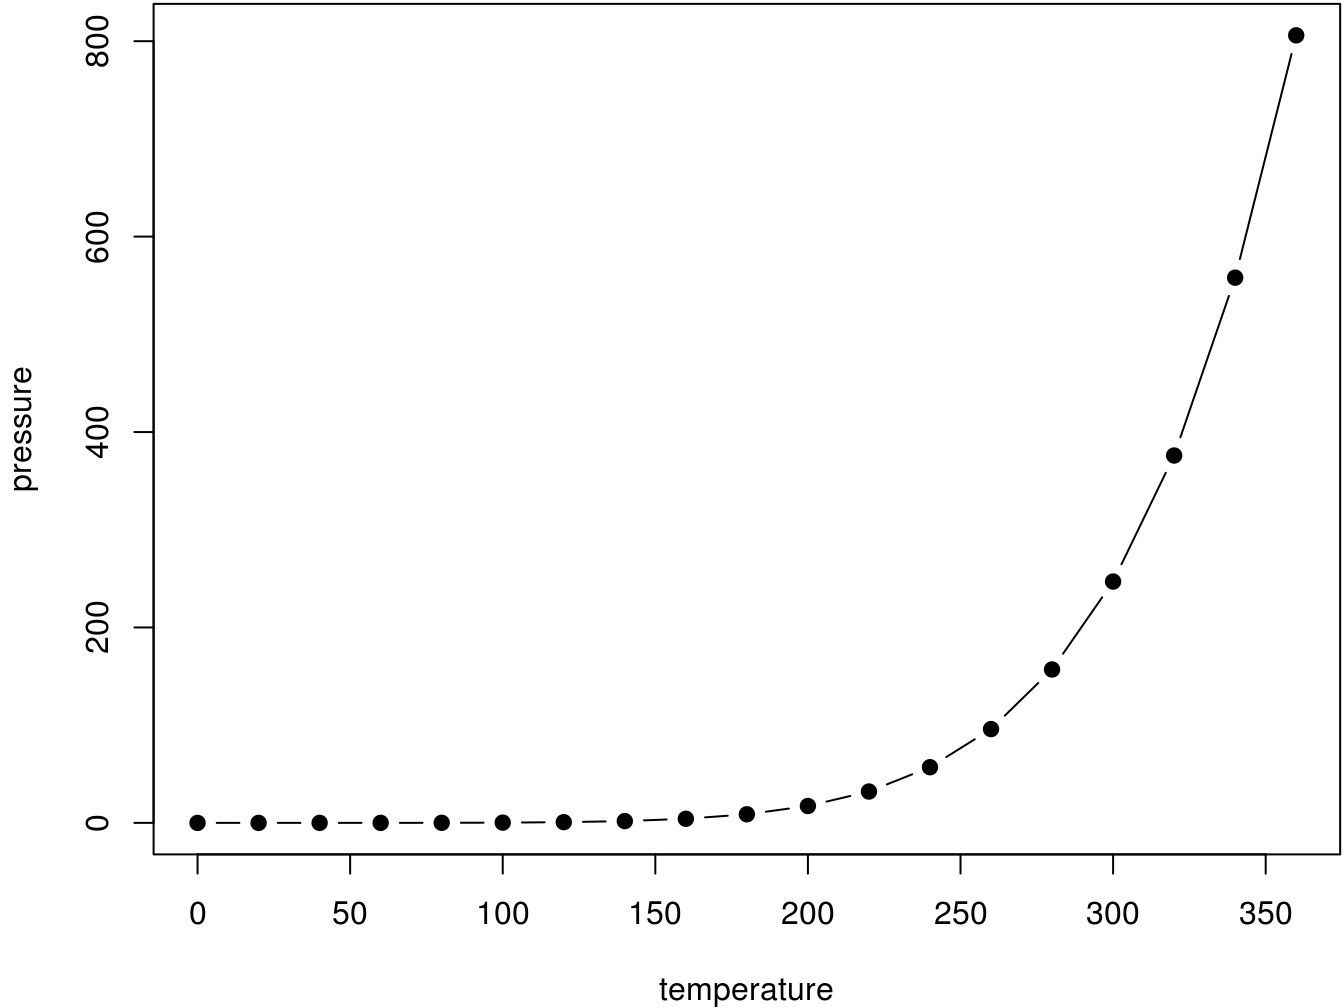
\includegraphics[width=0.8\linewidth]{bookdown-demo_files/figure-latex/nice-fig-1} 

}

\caption{Here is a nice figure!}\label{fig:nice-fig}
\end{figure}

Reference a figure by its code chunk label with the \texttt{fig:} prefix, e.g., see Figure \ref{fig:nice-fig}. Similarly, you can reference tables generated from \texttt{knitr::kable()}, e.g., see Table \ref{tab:nice-tab}.

\begin{Shaded}
\begin{Highlighting}[]
\NormalTok{knitr}\OperatorTok{::}\KeywordTok{kable}\NormalTok{(}
  \KeywordTok{head}\NormalTok{(iris, }\DecValTok{20}\NormalTok{), }\DataTypeTok{caption =} \StringTok{'Here is a nice table!'}\NormalTok{,}
  \DataTypeTok{booktabs =} \OtherTok{TRUE}
\NormalTok{)}
\end{Highlighting}
\end{Shaded}

\begin{table}

\caption{\label{tab:nice-tab}Here is a nice table!}
\centering
\begin{tabular}[t]{rrrrl}
\toprule
Sepal.Length & Sepal.Width & Petal.Length & Petal.Width & Species\\
\midrule
5.1 & 3.5 & 1.4 & 0.2 & setosa\\
4.9 & 3.0 & 1.4 & 0.2 & setosa\\
4.7 & 3.2 & 1.3 & 0.2 & setosa\\
4.6 & 3.1 & 1.5 & 0.2 & setosa\\
5.0 & 3.6 & 1.4 & 0.2 & setosa\\
\addlinespace
5.4 & 3.9 & 1.7 & 0.4 & setosa\\
4.6 & 3.4 & 1.4 & 0.3 & setosa\\
5.0 & 3.4 & 1.5 & 0.2 & setosa\\
4.4 & 2.9 & 1.4 & 0.2 & setosa\\
4.9 & 3.1 & 1.5 & 0.1 & setosa\\
\addlinespace
5.4 & 3.7 & 1.5 & 0.2 & setosa\\
4.8 & 3.4 & 1.6 & 0.2 & setosa\\
4.8 & 3.0 & 1.4 & 0.1 & setosa\\
4.3 & 3.0 & 1.1 & 0.1 & setosa\\
5.8 & 4.0 & 1.2 & 0.2 & setosa\\
\addlinespace
5.7 & 4.4 & 1.5 & 0.4 & setosa\\
5.4 & 3.9 & 1.3 & 0.4 & setosa\\
5.1 & 3.5 & 1.4 & 0.3 & setosa\\
5.7 & 3.8 & 1.7 & 0.3 & setosa\\
5.1 & 3.8 & 1.5 & 0.3 & setosa\\
\bottomrule
\end{tabular}
\end{table}

You can write citations, too. For example, we are using the \textbf{bookdown} package \citep{R-bookdown} in this sample book, which was built on top of R Markdown and \textbf{knitr} \citep{xie2015}.

\hypertarget{the-supply-and-demand-model}{%
\chapter{The Supply and Demand Model}\label{the-supply-and-demand-model}}

This unit focuses on the Supply and Demand model, a theoretical tool that shows how prices are shaped by the market interaction of sellers and buyers. Its malleability and simplicity makes this the most widely used model in economics. You can use the model to analyze a wide variety of markets: markets for consumer goods and services, financial markets, healthcare and insurance markets, labor markets among others.

By the end of this unit you will be able to:
1. Formulate conjectures on the source of price variations and identify data you could use to test these conjectures.
1. Use mathematical formalizations (equations and graphs) to represent the Supply and Demand model and to analyze and evaluate how economic shocks affect prices.
1. Use the Supply and Demand model to analyze the outcomes of various public policies.
1. Clearly explain your economic reasoning demonstrating fluency in Supply and Demand terminology.

\hypertarget{the-model}{%
\section{The model}\label{the-model}}

Goals are:
1. Explain and forecast price differences and changes
1. Predict the outcome and welfare effect of public policies
1. Evaluate whether public intervention could enhance market outcomes.

\hypertarget{supply-definition}{%
\subsection{Supply Definition}\label{supply-definition}}

The \textbf{direct relationship} between a product's \textbf{price and the quantity people (or organizations) wish to sell}.

\[Q_s = S(P,.,.) \quad S_p > 0\]
where \(P.,.,\) represents other variables such as opportunity cost, technology, information etc. These all shift the relationship.

\hypertarget{supply-definition-1}{%
\subsection{Supply Definition}\label{supply-definition-1}}

The \textbf{direct relationship} between a product's \textbf{price and the quantity people (or organizations) wish to buy}.

\[
Q_D = D(P,.,.,.,) \quad \text{and} \quad S_p >0
\]

where \(P,.,.\) represents other variables such as budget, substitutes availability, information, etc. that shift the relationship.

\hypertarget{purchasing-power}{%
\subsubsection{Purchasing Power}\label{purchasing-power}}

Normal goods:

Inferior Goods:

\hypertarget{related-goods}{%
\subsubsection{Related Goods}\label{related-goods}}

\begin{itemize}
\tightlist
\item
  \textbf{Gross Substitute:} something here
\item
  \textbf{Gross Compliments:} When the price of the compliment increases, then demand will decline (think gasoline and tires).
\item
  \textbf{Expected future prices:} If we think the price of an item will go up, we will want to buy more of this item today.
\item
  \textbf{Taxes:} Suppose government introduces a unit tax (of \(t\) dollars) on top of the price, known as a buyers tax. What will happen to the demand of the product? Demand will shift inward. Note that consumers can react differently to value-added-taxes compared to other taxes.
\end{itemize}

\hypertarget{equilibrium}{%
\subsubsection{Equilibrium}\label{equilibrium}}

The market is in equilibrium when there is no upward or downward pressure on prices.
That is when the quantity supplied equals the quantity demanded, and the market clears.

\hypertarget{comparative-statics}{%
\section{Comparative Statics}\label{comparative-statics}}

\hypertarget{the-formulas}{%
\subsection{The Formulas}\label{the-formulas}}

Suppose demand is \[Q_D = D(P, A, ...)\]
where \(P\) is a unit price and \(A\) a demand side Market condition (for example: income price of a substitute, a buyers tax\ldots)

and supply is: \$\$Q\_S = S(P,B,\ldots) where \(P\) is a unit price and \(B\) a demand side Market condition (for example: cost of labor, technology, a seller tax,\ldots)

\hypertarget{demand-side}{%
\subsubsection{Demand Side}\label{demand-side}}

INSERT A BUNCH OF STUFF

\hypertarget{example}{%
\paragraph{Example}\label{example}}

In the market for coffee:
\[Q_D = 300 - 20P + 10P_{tea} \quad \text{and} \quad Q_S = 20P-100 - 2(Wage)\]

Price of tea is a demand side market condition so we need to use the demand side formula. The change in price is 2 dollars (found in the demand function at \(+10P_{tea}\)). How senstive it is to coffee is in supply (\(+20\)). How sensitive it is to demand is in front of demand (\(-20\)).

So we end with: \[\frac{+10}{+20 - (-20)}\cdot 2 = \frac{1}{4} \cdot 2 = 50 cents\]

If it is a tax, a sellers tax, salience will 100 and we use the supply side formula. If it is a buyers tax, it is not always fully salient so we might have to take into account saliency.

\hypertarget{deriving-the-formula}{%
\subsubsection{Deriving the formula}\label{deriving-the-formula}}

\begin{enumerate}
\def\labelenumi{\arabic{enumi}.}
\tightlist
\item
  We start at equilibrium condition:
  \[Q_D(P*) = Q_S(P*)\]
  Equilibrium price itself and quantity is responsive to market conditions.
\item
  We highlight that equilibrium price depends on market condition A: \[Q*_D(P*(A),A_1,...) = Q*_S(P*(A),)\]
\item
  We differentiate both sides of the equilibrium condition respect to market condition A: \[ \frac{d}{dA} Q*_D(P*(A),A_1,...) = \frac{d}{dA} Q*_S(P*(A),)\]
  \[D_P \frac{dP*}{dA} + D_A =  S_P \frac{dP*}{dA}\]
  \[D_A =  S_P \frac{dP*}{dA} - D_P \frac{dP*}{dA}\]
  \[D_A = (S_P - D_P)\frac{dP*}{dA}\]
  \[dA \frac{D_A}{S_P - D_P} = dP*\]
\end{enumerate}

\hypertarget{derive-the-formula-for-supply-side-shock}{%
\subsubsection{Derive the formula for supply-side shock}\label{derive-the-formula-for-supply-side-shock}}

\[Q_D(P*) = Q_S(P*)\]
Now we highlight equilibrium:
\[Q*_D(P*(B)) = Q*_S(P*(B))\]
\[D_P \frac{dP*}{dB} = S_P \frac{dP*}{dB} + S_B\]

We need to get:
\[dD* = \frac{-S_B}{S_P - D_P}dB\]

So we see why they are cool, you can calculate interesting info without knowing exactly what the market is doing right now (as long as we have previous estimates).

The formulas work about the same in elasticity terms as well. We are in percent changes rather than absolute changes.

\[dP* = \frac{D_A}{S_P - D_P} \cdot dA\]
\[dP* = \frac{D_A \cdot A}{S_P - D_P} \cdot \frac{dA}{A}\]
Then divide by equilibrium quantity
\[dP* = \frac{D_A \cdot A/Q*}{S_P/Q* - D_P/Q*} \cdot \frac{dA}{A}\]
Divide both sides of the equation by equilibrium price:

\[\frac{dP*}{P*} = \frac{D_A \cdot A/Q*}{S_P/Q* - D_P/Q* \cdot P*} \cdot \frac{dA}{A}\]

Now what are each term:
- Numerator on right is a demand elasticity to changes in A.
- Left half the denominator is price elasticity of supply
- Right half of the denominator is the price elasticity of demand
- left half is percentage change in price

\[ \perc \delta P = \frac{\Epsilon_A^D}{M_P^S - something else}\]

\hypertarget{explain}{%
\paragraph{Explain}\label{explain}}

True or false? Markets where demand and supply are relatively price inelastic display higher price volatility.

It is true of course. First you can look at graphs with a supply shift. With a flat demand curve (elastic), then there is no change in price; but, when you use an inelastic demand curve, then there is a huge change in price.

Similarly: we can look at the formula we just did;

INSERT THING!

\#\#\#Overview:

Demand is a negative function of price and many other things.

Supply is a positive function of price and many other things.

We want to find equilibrium prices and quantities. We believe the the price is driven by the market wanting to balance quantity demanded and supplied.

We also know the formulas from the last half and use calculus and elasticity. We can see what happens to the prices when market conditions change. If we want magnitude we use calculus. If we want just absolute change we can graph it.

We learned about taxation. Taxation incidence, how much the different buyers and sellers share the price of the tax. We learned that whether you collect a buyers or sellers tax actually matters for salience.

\hypertarget{consumer-choice}{%
\chapter{Consumer Choice}\label{consumer-choice}}

This module focuses on the Consumer Choice model. The model captures how rational consumers allocate their budgets of money or time among different valuable uses. The model is quite flexible and economists use it to analyze how shoppers decide what to buy, how families decide how much to save, or how workers decide whether to look for a job or how many hours they wish to spend working. The ultimate goal of the model is to help us understand how changes in economic conditions, including public policy, influence these very important decisions.

\begin{enumerate}
\def\labelenumi{\arabic{enumi}.}
\tightlist
\item
  Use algebra and graphs to represent consumers' economic predicament and the trade-offs they face
\item
  Capture and illustrate the key features of consumers' tastes with utility functions and indifference curves
\item
  Apply the Lagrangian method to determine consumers' optimal choices
\item
  Explain when a consumer is in equilibrium and why at times consumers don't purchase items even if these are affordable
\end{enumerate}

How do you work like an economist?

\begin{enumerate}
\def\labelenumi{\arabic{enumi}.}
\tightlist
\item
  You start by noticing some anecdotal facts
\item
  You collect data (or review existing ones) to verify there are some more general regularities
\item
  You form a theoretical conjecture that could explain the empirical evidence
\item
  You build a formal model that illustrates your conjecture
\item
  You use statistical methods to:
\end{enumerate}

\begin{enumerate}
\def\labelenumi{\alph{enumi})}
\tightlist
\item
  Evaluate the magnitude of the parameters driving your model
\item
  Test if your model matches the empirical evidence
\item
  Test the direction of causality between variables
\item
  Forecast future developments and/or effects of policy intervention.
\end{enumerate}

Think like an economicst on economic models:
1. You contrust a simplified description of conditions under which people take actions
2. Then you describe in simple terms what drives the action that people take
3. You determine how each of their actions affects each other
4. Determine the outcomes of these actions. This is often an equilibrium
5. You try to get more insight by studying what happens to key variables when certain conditions change.

\hypertarget{applications}{%
\chapter{Applications}\label{applications}}

Some \emph{significant} applications are demonstrated in this chapter.

\hypertarget{example-one}{%
\section{Example one}\label{example-one}}

\hypertarget{example-two}{%
\section{Example two}\label{example-two}}

\hypertarget{final-words}{%
\chapter{Final Words}\label{final-words}}

We have finished a nice book.

\hypertarget{something-something}{%
\chapter{Something something}\label{something-something}}

\hypertarget{test-review}{%
\chapter{Test Review}\label{test-review}}

  \bibliography{book.bib,packages.bib}

\end{document}
